%==============================================================================
% MM_paper_IEEE.tex -- IEEE BIBM 2026 camera-ready (IEEEtran, US Letter).
%   pdflatex MM_paper_IEEE ; pdflatex MM_paper_IEEE
%==============================================================================
\pdfminorversion=4   % PDF 1.4 (Acrobat 5 compatible) for IEEE PDF eXpress
\documentclass[conference,letterpaper]{IEEEtran}
\IEEEoverridecommandlockouts
\usepackage[utf8]{inputenc}
\usepackage{cite}
\usepackage{graphicx}
\usepackage{booktabs}
\usepackage{array}
\usepackage{amsmath,amssymb}
\usepackage{xcolor}
\usepackage{listings}
\usepackage[hidelinks]{hyperref}
\usepackage{newtxtext,newtxmath}   % Times (Type 1, embeddable)

\lstset{basicstyle=\ttfamily\scriptsize,breaklines=true,frame=single,
        language=Verilog,columns=fullflexible,keepspaces=true}

\title{Mutations as Stuck-at Faults: A Logic-Circuit and Finite-State-Machine
Formalization of Boolean Cancer Signaling Networks, with HDL Export ---
A Multiple Myeloma Case Study}

\author{%
\IEEEauthorblockN{Sang Hoon Chung\IEEEauthorrefmark{1},
Madhurima Mondal\IEEEauthorrefmark{1},
Norman Reeves\IEEEauthorrefmark{2}, and
Aniruddha Datta\IEEEauthorrefmark{1}}
\IEEEauthorblockA{\IEEEauthorrefmark{1}\textit{Dept.\ of Electrical and Computer Engineering},
\textit{Texas A\&M University}, College Station, TX, USA\\
hunkun1@tamu.edu, mmkpa2012@tamu.edu, datta@ece.tamu.edu}
\IEEEauthorblockA{\IEEEauthorrefmark{2}\textit{Sumaq Life LLC}, Columbus, OH 43206, USA\\
peter.reeves@sumaqlife.com}
}
% IEEE copyright notice: add ONLY if the eCF/BIBM instructions give you a line, e.g.
% \IEEEpubid{\makebox[\columnwidth]{979-8-XXXX-XXXX-X/26/\$31.00~\copyright2026 IEEE \hfill}
% \hspace{\columnsep}\makebox[\columnwidth]{ }}

\begin{document}
\maketitle

\begin{abstract}
Boolean network models of cancer signaling are interpretable but are usually
analyzed as bespoke dynamical systems, seldom with the mature theory and tooling
of digital logic design. Building on the pathway-logic and test-generation
formulation of cancer therapy, in which an oncogenic mutation is a
\emph{stuck-at fault}, a drug is an \emph{input} that masks faults, and a drug
combination is a \emph{multi-fault test pattern}, we formalize a multiple myeloma
(MM) signaling network as a logic circuit. A single-pass (combinational) model
reproduces the standard bortezomib--dexamethasone--lenalidomide (VRd) backbone;
restoring the IRF4--MYC positive feedback loop and an absorbing apoptosis latch
turns the circuit into a synchronous \emph{sequential circuit} / finite-state
machine (FSM) whose attractors are cell fates. Across $352$ regimen-by-fault
conditions, $24\%$ are multistable---invisible to the single-pass model---and
multistability falls from $41\%$ under single agents to $5\%$ under quadruplets,
so combinations remove the dependence of outcome on the prior cell state.
Monte-Carlo confidence intervals show that, by construction, the two anti-CD38
antibodies are indistinguishable ($\Delta=0.0003$, $95\%$ CI $[-0.019,0.020]$).
Without being fit to outcomes, the model reproduces the VRd standard of care and
the clinically recognized high-risk genotypes, and its regimen ranking is robust
to the update scheme, individual rules, and readout; we present these rankings as
\emph{in silico} mechanistic hypotheses. Finally, we export the FSM as
\emph{synthesizable Verilog} with stuck-at fault ports, verified equivalent to
the reference model on $20{,}000$ random cases, as a standard interface to
electronic-design-automation verification and test-generation tools.
\end{abstract}

\begin{IEEEkeywords}
Boolean networks, attractors, multiple myeloma, stuck-at faults,
finite-state machines, Verilog, drug combinations
\end{IEEEkeywords}

%==============================================================================
\section{Introduction}\label{sec:intro}
Multiple myeloma (MM) is a malignant clonal proliferation of bone-marrow plasma
cells and one of the most common hematologic malignancies~\cite{seer,acs,globocan}.
Two decades of novel agents have markedly improved outcomes, yet MM remains
\emph{incurable}: essentially all patients relapse, with clonal evolution and
multi-drug resistance~\cite{relapse}. The central clinical question has therefore
shifted from \emph{whether} to treat toward \emph{which} combination, in
\emph{which} order, for a genetically heterogeneous patient.

Modern therapy combines several mechanistically distinct drug classes, and the
introduction of proteasome inhibitors, immunomodulatory drugs (IMiDs), and
anti-CD38 antibodies has repeatedly raised the standard of care; quadruplet
regimens now outperform triplets in newly diagnosed disease~\cite{perseus}.
Precisely because the disease is heterogeneous and relapsing, however, the
number of clinically reasonable regimen-and-sequence choices is large, and
selecting among them for an individual patient remains largely empirical.

Frontline care draws on a small set of building blocks---a proteasome inhibitor
(e.g., bortezomib), an IMiD (e.g., lenalidomide), a corticosteroid
(dexamethasone), and increasingly an anti-CD38 antibody (daratumumab or
isatuximab)---assembled into backbones such as VRd and the quadruplet
D-VRd~\cite{perseus}. Even this short list yields dozens of combinations, and
the space grows once mutational context and line of therapy are considered.
Mechanistic, interpretable models that predict how a given combination acts on a
given genotype are therefore attractive as decision-support tools.

Boolean and logic-based network models suit this setting because they are
interpretable and need few quantitative parameters; prior work has recapitulated
MM regimens and even predicted clinical response~\cite{cbm,fumia}. Our starting point is the pathway-logic line of work
in which a mutation is a \emph{stuck-at fault} and therapy is fault
correction~\cite{layek,gsp}, therapy design is Max-SAT-based automatic
test-pattern generation (ATPG)~\cite{linkhatri}, and model-predicted combinations
have been tested experimentally in colorectal cancer~\cite{vundavilli}. We adopt
that formulation rather than claim it (Fig.~\ref{fig:overview}).

\noindent\textbf{Contributions.} Building on this foundation, we contribute three
things:
\begin{itemize}\itemsep2pt
  \item \textbf{An integrated MM network} (ten pathways, $22$ nodes, $22$ faults,
  five drugs) in the stuck-at-fault vocabulary, with an exhaustive
  combinational-equivalence check of its gate netlist (Sec.~\ref{sec:comb}).
  \item \textbf{An explicit feedback / attractor analysis}: the IRF4--MYC loop and
  an absorbing apoptosis latch make the circuit a sequential FSM, and we
  \emph{quantify}, by exact enumeration, the multistability this adds over the
  single-pass score, interpret it biologically, and show which predictions it
  changes (Secs.~\ref{sec:attr}, \ref{sec:res-attr}).
  \item \textbf{A synthesizable Verilog realization} of the FSM with stuck-at
  ports, verified equivalent to the reference model, that exposes the network to
  standard EDA tools without re-encoding (Sec.~\ref{sec:hdl}).
\end{itemize}
We complement these with Monte-Carlo uncertainty quantification, baselines and
null models, robustness analyses, an exhaustive ATPG demonstration, and a
literature-concordance check, and we specify a protocol for external validation
(Secs.~\ref{sec:val}, \ref{sec:results}).

\begin{figure*}[t]
\centering
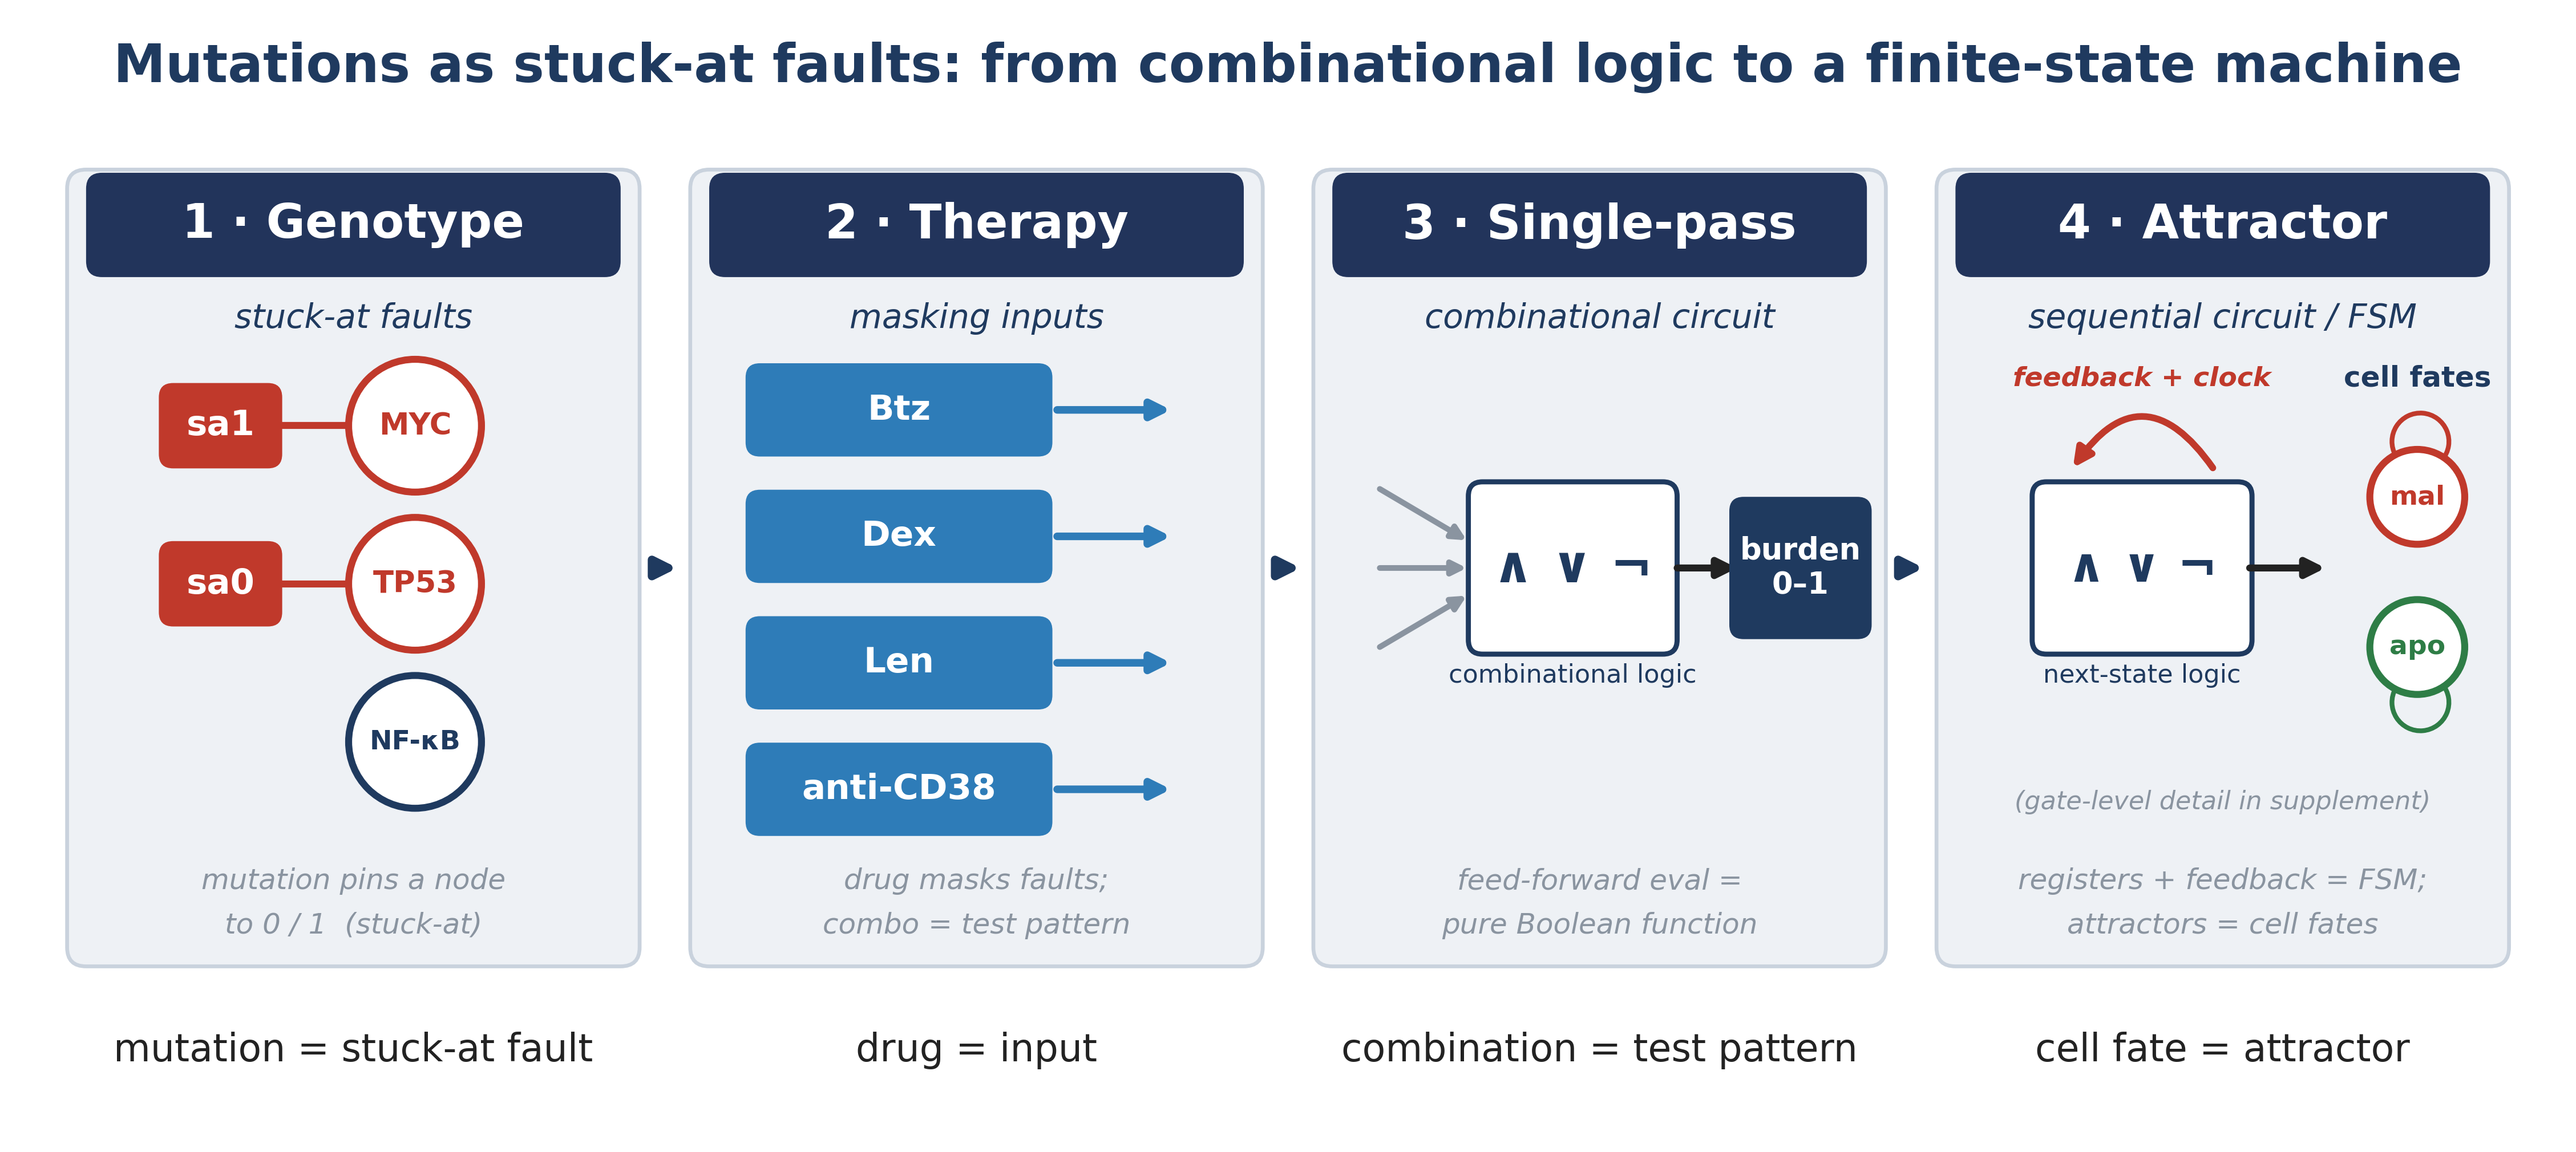
\includegraphics[width=0.99\textwidth]{MM_figure1_overview.png}
\caption{Overview of the formalism. A genotype pins network nodes as stuck-at
faults (stage 1); drugs are inputs that mask faults, and a combination is a
multi-fault test pattern (stage 2). Evaluated feed-forward, the network is a
combinational circuit whose output is an oncogenic-burden score (stage 3);
adding registers and feedback makes it a sequential circuit / finite-state
machine whose attractors are cell fates (stage 4). Bottom: the core analogy.}
\label{fig:overview}
\end{figure*}

%==============================================================================
\section{Background and Related Work}\label{sec:bg}

\textbf{MM signaling.} Survival signals converge on NF-$\kappa$B (canonical and
non-canonical, via TNF/RANK/NIK), which sustains the anti-apoptotic guards MCL1
and BCL-xL; IL-6/JAK/STAT3 signaling reinforces the same program and confers
apoptosis resistance~\cite{stat3}. A defining feature of MM is the IRF4--MYC
autoregulatory loop, an addiction of the malignant clone~\cite{shaffer}.
Proliferation runs through cyclin~D/CDK4/6/E2F with PI3K/AKT/mTOR and RAS/MAPK as
parallel inputs, and the apoptotic decision is set by the BCL-2 family balance
(NOXA/BIM versus MCL1/BCL-xL) and p53. Bortezomib blunts NF-$\kappa$B and induces
NOXA; dexamethasone induces BIM; lenalidomide engages CRBN to degrade IKZF1/3 and
collapse IRF4--MYC~\cite{kronke}; anti-CD38 antibodies act predominantly through
immune effectors. Pathways are assembled from KEGG~\cite{kegg}.

\textbf{Boolean networks and digital logic.} A Boolean network abstracts each
species to ON/OFF and each rule to a logic function; iterated from an initial
state it settles into an \emph{attractor} (fixed point or cycle), read as a cell
phenotype~\cite{kauffman}. Positive feedback is necessary for
multistability~\cite{thomas}. Attractors are computed by tools such as PyBoolNet,
GINsim, and MaBoSS~\cite{pyboolnet,ginsim,maboss}, exactly via SAT-based methods
for synchronous networks~\cite{dubrova}. In digital design, a feed-forward network
is a \emph{combinational} circuit; the \emph{stuck-at fault} model ties a wire to
$0$ or $1$, and ATPG searches for inputs that expose faults~\cite{testing}; with
feedback and registers the circuit is \emph{sequential}---an FSM whose reachable
states and cycles are its attractors. Hardware description languages (HDLs) such
as Verilog describe FSMs for simulation, equivalence checking, and model checking.

\textbf{Related work and positioning.}
Boolean models of cancer signaling are well established: Fum\`ia and Martins
built a Boolean model spanning cancer-hallmark pathways~\cite{fumia}, and
multiscale frameworks such as PhysiBoSS couple Boolean signaling to agent-based
cell populations~\cite{physiboss}. In MM specifically, constraint-based and
logic models have recapitulated and even predicted response to RVd-type
regimens~\cite{cbm}. General-purpose tools---BoolNet, PyBoolNet, GINsim, MaBoSS,
and the data-driven CellNOpt---support attractor computation, model reduction,
and rule inference~\cite{pyboolnet,ginsim,maboss,cellnopt}. Closest to our work, Layek et al.\ modeled cancer growth-factor pathways as
Boolean logic circuits and cast mutations as stuck-at faults for therapy
design~\cite{layek}, within the genomic-signal-processing program of Dougherty
and Datta~\cite{gsp}. Lin and Khatri solved therapy design as Max-SAT ATPG on such
circuits and sketched a sequential, time-frame-expanded formulation that uses
attractor states~\cite{linkhatri}. Vundavilli et al.\ applied a Boolean model to
multiple mutations and drug combinations in colorectal cancer and tested the
predicted combinations in HT29 and HCT116 cells~\cite{vundavilli}. Relative to
these, we contribute no new fault or ATPG formulation. We (i)~build and audit an
integrated MM model; (ii)~make the feedback/attractor extension explicit for a
disease network and \emph{measure} what it changes relative to the single
pass---Lin and Khatri use attractor states inside the ATPG encoding but do not
quantify multistability or its effect on regimen rankings; and (iii)~realize the
model as a synthesizable HDL artifact rather than an internal CNF encoding, so
that unmodified EDA tools can consume it. Unlike Vundavilli et al., our
predictions have not yet been tested experimentally, and we treat them as
hypotheses.

%==============================================================================
\section{Methods}\label{sec:methods}

The method has four parts that mirror Fig.~\ref{fig:overview}: a curated network
(Sec.~\ref{sec:net}), a combinational fault formalism (Sec.~\ref{sec:comb}), a
dynamical attractor model (Sec.~\ref{sec:attr}), and a sequential-circuit / HDL
realization (Sec.~\ref{sec:hdl}).

\subsection{Network construction and provenance}\label{sec:net}
We integrate ten KEGG pathways~\cite{kegg} into a single MM signaling network---%
NF-$\kappa$B (hsa04064), PI3K--AKT (hsa04151), JAK--STAT (hsa04630), RAS/MAPK
(hsa04014), Wnt (hsa04310), proteasome (hsa03050), apoptosis (hsa04210), cell
cycle (hsa04110), transcriptional misregulation (hsa05202), and calcium
(hsa04020)---joined at shared hubs (NF-$\kappa$B survival, the
ubiquitin--proteasome axis, the RTK/RAS/PI3K backbone, the BCL-2-family apoptosis
node, the c-Myc/cyclin-D relay, p53, and the MM-specific IgH-translocation root).
Each node carries a Boolean rule $x_i^{+}=f_i(\mathbf{x},\mathbf{u})$ over its
regulators and the drug/context inputs $\mathbf{u}$; each rule is an explicit,
auditable choice, not parameter-fit. The network has $22$ internal nodes and $8$
oncogenic readouts, driven by $5$ drug inputs; microenvironmental inputs (IL-6,
IGF-1, RANKL, Wnt, hypoxia, TNF) are held at their resting baseline so the score
reflects intrinsic, drug-modulated signaling. Forty-nine edges terminate on the
internal nodes ($38$ internal---one the APOP self-loop of the absorbing
latch---plus $8$ drug-action and $3$ PTEN/CRBN context edges), and $5$ more
produce the readouts (ANTIAPOP $=$ MCL1$\vee$BCL-xL, VEGF, SURVIVAL). The drugs
act at bortezomib\,$\to$\,26S proteasome (I$\kappa$B, NOXA),
dexamethasone\,$\to$\,glucocorticoid receptor (BIM),
lenalidomide\,$\to$\,CRL4--CRBN (IKZF1/3\,$\to$\,IRF4--MYC)~\cite{kronke}, and
anti-CD38\,$\to$\,CD38.


\subsection{Combinational formalization}\label{sec:comb}
In the single-pass model the nodes are evaluated once in topological order, so
the mapping from inputs to the eight readouts is a pure Boolean function --- a
combinational circuit of AND/OR/NOT gates. We give the three biological objects a
common logic-design meaning. A \emph{stuck-at fault} pins node $i$ to a constant
$c\in\{0,1\}$, overriding its rule ($x_i\equiv c$); this encodes an oncogenic
lesion (e.g., NF-$\kappa$B stuck-at-$1$, or TP53/PTEN stuck-at-$0$). A drug is an
input that \emph{masks} faults by forcing or gating specific nodes (e.g.,
bortezomib drives $\text{NFKB}\!\to\!0$ and $\text{NOXA}\!\to\!1$; dexamethasone
induces BIM; lenalidomide, when CRBN is intact, collapses IRF4 and raises p21),
so a fault may be observable, partially masked, or fully corrected at the
readout. A drug combination is then a \emph{multi-fault test pattern} --- the
joint input applied against a possibly multi-fault genotype. Anti-CD38 is modeled
only by its cell-intrinsic, Fc-independent pro-apoptotic input, subject to the
same BH3 guards; its dominant immune-effector mechanism (ADCC/CDC) is
cell-extrinsic and out of scope for this intrinsic model.

Faults are realized as multiplexers built from the same primitives: a node with a
stuck-at select becomes $\mathrm{OR}(x_i,\mathrm{sel})$ for stuck-at-$1$ and
$\mathrm{AND}(x_i,\lnot\mathrm{sel})$ for stuck-at-$0$. We checked the gate
netlist against the rule-based reference exhaustively: all baseline and
single-fault conditions ($23$) together with all fault pairs
($\binom{22}{2}=231$), each crossed with the $2^{5}=32$ on/off drug
combinations---i.e., $(23+231)\times 32 = 8{,}128$ cases. On every case the
gate netlist reproduces the rule-based reference exactly---zero mismatches, i.e.
no input for which the two implementations' $8$-bit outputs differ.

\subsection{Dynamical (attractor) model}\label{sec:attr}
To capture cell-fate multistability we restore the feedback that the single pass
omits and switch to state-based dynamics. Three changes distinguish this model
from the combinational one. The IRF4--MYC positive feedback loop is closed
($\text{IRF4}^{+}=\lnot\text{Len}_{\text{active}}\wedge(\text{NFKB}\vee\text{MYC})$
and $\text{MYC}^{+}=\text{IRF4}\wedge(\text{ERK}\vee\text{BCAT}\vee\text{STAT3}
\vee\text{NFKB}\vee\text{MTOR})$); survival is coupled to the loop
($\text{MCL1}^{+}=\text{STAT3}\vee\text{NFKB}\vee\text{IRF4}$); and apoptosis is
an \emph{absorbing} latch
($\text{APOP}^{+}=\text{APOP}\vee(\text{pro}\wedge\lnot\text{guarded})$, with
$\text{pro}=\text{NOXA}\vee\text{BIM}\vee\text{antiCD38}$ and $\text{guarded}$ the
unopposed BH3-guard term), so commitment to death is irreversible; the latch encodes mitochondrial
outer-membrane permeabilization, widely regarded as the point of no return of
intrinsic apoptosis~\cite{tait}. These edges
make the influence graph cyclic---exactly what multistability
requires~\cite{thomas}---whereas the single pass omits them and is acyclic.

All $22$ nodes are updated \emph{synchronously}. From each of $n_{\text{init}}$
initial states---drawn uniformly at random over the $22$ bits, with faulted
nodes pinned and $\text{APOP}=0$ (the cell starts alive)---we iterate the update
until a state recurs; the recurring set is the attractor (a fixed point or a
limit cycle), detected at first repetition. An attractor is \emph{apoptotic} if
any of its states has $\text{APOP}=1$. Each condition yields three readouts. The
\emph{apoptotic propensity} is the fraction of initial states reaching an
apoptotic attractor. The \emph{residual} burden averages, over initial states, a
per-cell load equal to $0$ for an apoptotic attractor and otherwise the mean over
the attractor's states of $(\text{oncogenic outputs ON})/8$, using the eight
readouts MYC, CCND2, E2F, NFKB, ANTIAPOP, VEGF (which equals STAT3 with hypoxia
off), CDK4/6, and SURVIVAL; dead cells thus contribute $0$ and living cells
contribute their program load. The number of distinct attractors indexes
multistability. Unless stated otherwise, $n_{\text{init}}=120$. Because the
environment inputs are fixed, every attractor lies in a $2^{16}$ alive-state
subspace, which we also enumerate exhaustively, so the attractor sets do not
depend on $n_{\text{init}}$.
As a robustness check we also evaluate the model under random-asynchronous
updating (one randomly selected node updated per step, with faulted nodes
pinned); the agreement with synchronous results is reported in
Sec.~\ref{sec:res-sens}.

\subsection{Sequential circuit and HDL export}\label{sec:hdl}
With feedback and a clock the model is a finite-state machine (FSM): the state is
a $22$-bit register $Q$ (one D flip-flop per node), the next-state logic is the
combinational netlist of Sec.~\ref{sec:comb} augmented with the restored feedback,
a fault is a constant tie on a state bit, and a drug
is an input pin. The FSM's reachable states and cycles are exactly the attractors
of Sec.~\ref{sec:attr}. We export this machine as synthesizable Verilog;
the exported module \texttt{mm\_attractor} (listing in the online supplement) exposes
\texttt{clk} and \texttt{load}, an \texttt{init[21:0]} seed, the five drug pins
(\texttt{Isa}, \texttt{Dara}, \texttt{Btz}, \texttt{Dex}, \texttt{Len}),
context/fault flags (\texttt{PTEN}, \texttt{CRBN}, \texttt{BIM\_del}), a per-node
stuck-at interface (\texttt{sa\_en[21:0]}, \texttt{sa\_val[21:0]}), and outputs
\texttt{Q[21:0]} with the decoded phenotypes \texttt{APOP\_out} and
\texttt{SURVIVAL\_out}. A self-checking testbench, run in the open-source
Icarus Verilog simulator, applies $20{,}000$ random state/fault/drug vectors and
finds zero mismatches against the Python reference (a deliberately removed gate
yields $1{,}029$). This establishes that the translation is correct; it is an
engineering contribution that makes the model consumable by EDA tools, not by
itself a faster analysis. This FSM view
also makes drug-combination search an automatic-test-pattern-generation problem,
which we exploit in Sec.~\ref{sec:res-atpg}.

\subsection{Drug screen, readout, and uncertainty}\label{sec:screen}
We screen regimens of up to four agents. For each regimen we compute the
attractor residual (Sec.~\ref{sec:attr}) against every single fault, every fault
pair, and every fault triple, average within each order, and rank regimens by the
mean; reporting the three orders separately shows how a regimen degrades as
genotypic complexity grows (Table~\ref{tab:rank}). Because initial conditions are
sampled, each residual is a Monte-Carlo estimate. For uncertainty we run $R=60$
independent replicates with distinct seeds, each averaging $n_{\text{init}}=60$
initial states over the $22$ single faults, and report the mean with a $95\%$
confidence interval taken as the $2.5$th and $97.5$th replicate percentiles
(Sec.~\ref{sec:res-ci}). The same procedure tests whether two regimens are
separable: the isatuximab-vs-daratumumab contrast is the paired per-replicate
difference, whose interval contains $0$ by construction because the intrinsic
model represents both antibodies with the single antiCD38 input.

\subsection{Validation, baselines, sensitivity}\label{sec:val}
The model is a mechanistic hypothesis, not a fitted classifier, so we specify a
validation design rather than a tuned result; the analyses below are stated here
and reported where available in Sec.~\ref{sec:results}.
\emph{(i) External validation.} Patient genotypes are mapped to stuck-at faults
and administered regimens to drug inputs, and the predicted apoptotic propensity
(Sec.~\ref{sec:attr}) is compared with the observed serum free-light-chain
($\kappa/\lambda$) response, scoring discrimination by AUC; as a fully public
alternative, predictions are tested against MM cell-line drug sensitivity in
DepMap/CTRP/GDSC.
\emph{(ii) Baselines and null models.} Predictions are compared with a
drug-count baseline (rank by number of agents only) and a randomized-rule null
(the same topology with operators/signs shuffled), to confirm that ranking skill
comes from the network logic rather than from regimen size or graph size alone.
\emph{(iii) Sensitivity.} We perturb the modeling choices on which the results
depend---swapping OR$\leftrightarrow$AND at multiplexed nodes, removing
individual edges, varying the readout set, and switching from synchronous to
asynchronous update---and report how the regimen ranking and the multistability
fraction move. Controls (ii) and (iii) are executed below (Sec.~\ref{sec:res-baseline}, Sec.~\ref{sec:res-sens}); the external validation (i) requires genotype-and-outcome data and remains future work.

%==============================================================================
\section{Results}\label{sec:results}

\subsection{Recapitulation of the standard backbone}\label{sec:res-vrd}
The top-ranked regimen is the VRd backbone, with anti-CD38 quadruplets nearly
tied (Table~\ref{tab:rank}), consistent with clinical practice.

\begin{table}[t]
\centering\small
\caption{Top regimens by the attractor model (lower mean $=$ better);
single/double/triple are mean attractor residuals over single faults, fault pairs, and fault triples, computed with a shared seed.
Regimens the intrinsic model encodes identically receive identical scores: adding
anti-CD38 to any bortezomib/dexamethasone backbone leaves the score unchanged
(Sec.~\ref{sec:res-ci}), so those rows are collapsed.}
\label{tab:rank}
\begin{tabular}{@{}lcccc@{}}
\toprule
Regimen & $n$ & single & double & triple \\
\midrule
(anti-CD38\,$\pm$)\,VRd & 3--4 & 0.008 & 0.028 & 0.062 \\
(anti-CD38\,$\pm$)\,Btz+Dex & 2--3 & 0.011 & 0.040 & 0.087 \\
\bottomrule
\end{tabular}
\end{table}

\subsection{Single-pass vs.\ attractor}\label{sec:res-attr}
Single-pass and attractor scores are correlated ($r=0.76$) but far from
identical (Fig.~\ref{fig:compare}): of the $352$ regimen-by-fault conditions,
$85$ ($24\%$) are multistable---invisible to the single pass---and $177$ ($50\%$)
differ from the single-pass burden by more than $0.1$ (mean $|\Delta|=0.117$).
Because the environment inputs are held fixed, every attractor lies in a $2^{16}$
alive-state subspace, so we enumerate the attractor set \emph{exhaustively}
rather than sampling it: the exact multistable fraction is $24.2\%$, equal to the
Monte-Carlo estimate (agreement on $95\%$ of conditions), so the sampling is not
missing attractors and the figure needs no confidence interval. Exact and
symbolic attractor enumeration is well established (e.g.\ SAT-based bounded model
checking~\cite{dubrova}); it is tractable here because the reachable subspace is
only $2^{16}$. On
average the attractor residual is \emph{lower} (mean $\Delta=-0.103$), because
cells that commit to the absorbing death state contribute zero; but in a minority
of conditions the restored feedback \emph{sustains} the oncogenic program and the
attractor model is \emph{more} malignant than the acyclic single pass would
predict---exactly the bistable-survival cases it cannot represent. STAT3-driven disease leaves the largest residual under
all four-drug regimens, since no agent targets STAT3. The full attractor heatmap
is provided as online supplementary material.

\begin{figure}[t]
\centering
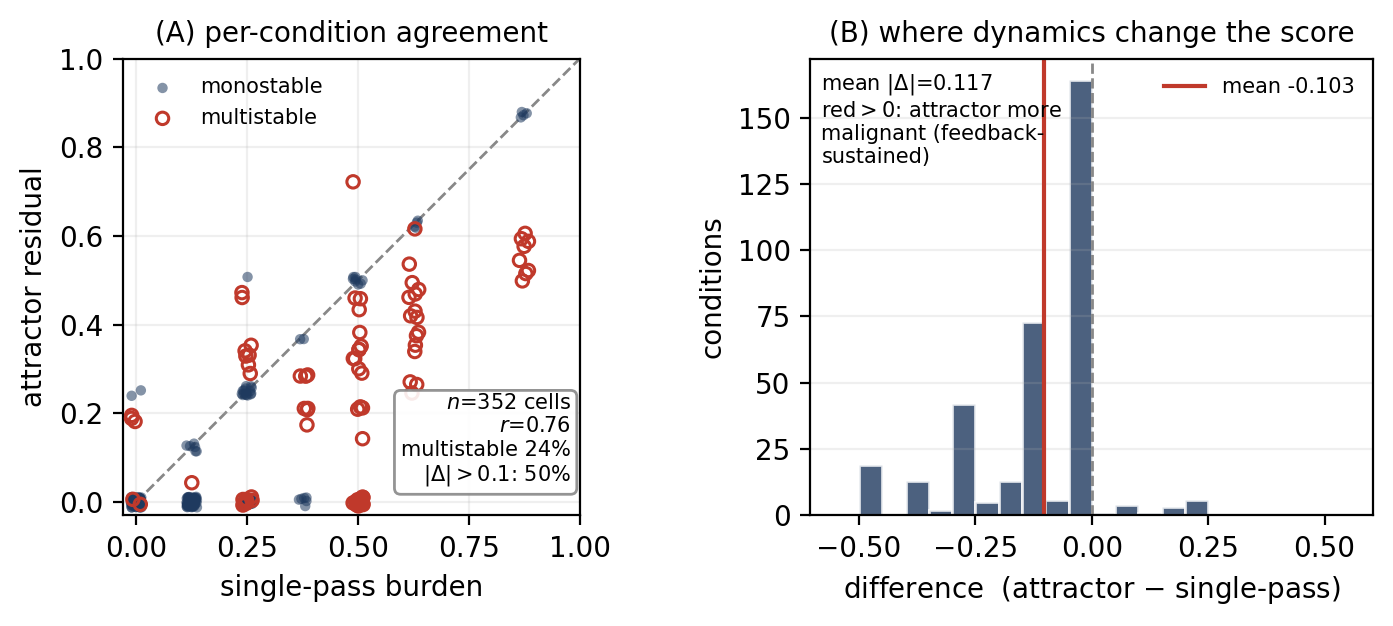
\includegraphics[width=\linewidth]{MM_compare_compact.png}
\caption{What the dynamical extension adds. (A) per-condition agreement between
the single-pass burden and the attractor residual; multistable conditions (red
rings) are invisible to the single-pass model. (B) distribution of the
difference: on average the attractor residual is lower (mean $\Delta=-0.103$,
since committed-apoptotic cells score zero), with a feedback-sustained tail that
is \emph{more} malignant than the single pass---the cases it misses
(mean $|\Delta|=0.117$).}
\label{fig:compare}
\end{figure}

The multistable conditions have a biological reading. In $55$ of the $85$
($65\%$), the same genotype and regimen lead to \emph{both} an apoptotic and a
surviving attractor, depending on the cell's prior state: fractional killing, a
mechanistic analogue of partial response. The surviving state is usually the
IRF4--MYC-ON program, the MM addiction state~\cite{shaffer}, or, under
lenalidomide, a loop-OFF state; constitutive STAT3 under VRd, for example, splits
about evenly. Another $24$ ($28\%$) differ only among death states and are
phenotypically equivalent, and $6$ ($7\%$) are alternative living states. The two
restored elements account for these effects: the latch generates the survive/die
splits (removing it lowers them from ${\sim}16\%$ to ${\sim}2\%$ of conditions),
and the IRF4--MYC loop half of the attractor multiplicity (removing MYC$\to$IRF4
lowers $24\%$ to $12\%$). The therapeutic prediction that changes is how state
dependence scales with combination size: multistability falls from $41\%$ of
conditions under single agents to $26\%$, $12.5\%$, and $4.5\%$ under two-,
three-, and four-drug regimens. Combinations thus act not only by lowering burden
but by removing history dependence, which the acyclic single pass cannot express.
The best single agent also changes (bortezomib in the dynamical model,
dexamethasone in the single pass).



\subsection{Uncertainty and same-target agents}\label{sec:res-ci}
Reporting each regimen with a $95\%$ confidence interval over $R=60$
Monte-Carlo replicates (Fig.~\ref{fig:ci}), the two anti-CD38 antibodies
overlap completely (Isatuximab $0.297$ $[0.285,0.311]$; Daratumumab $0.297$
$[0.283,0.309]$; difference $\Delta=0.0003$, $95\%$ CI $[-0.019,0.020]$). The
intrinsic model encodes both as one node, so any apparent difference is
sampling noise; with a shared seed the two are bit-identical. More strongly, the
intrinsic death rule is $\text{pro}=\text{NOXA}\vee\text{BIM}\vee\text{antiCD38}$
with bortezomib$\to$NOXA and dexamethasone$\to$BIM, so anti-CD38 is logically
\emph{subsumed}: it adds \emph{exactly zero} to any bortezomib- or
dexamethasone-containing backbone, and changes the score only in their absence
(e.g., untreated vs.\ anti-CD38 alone). The model therefore does not merely fail
to separate the two antibodies---within standard backbones it does not register
the antibody at all. This is a resolution limit of the intrinsic scope, not a
result.

\begin{figure}[t]
\centering
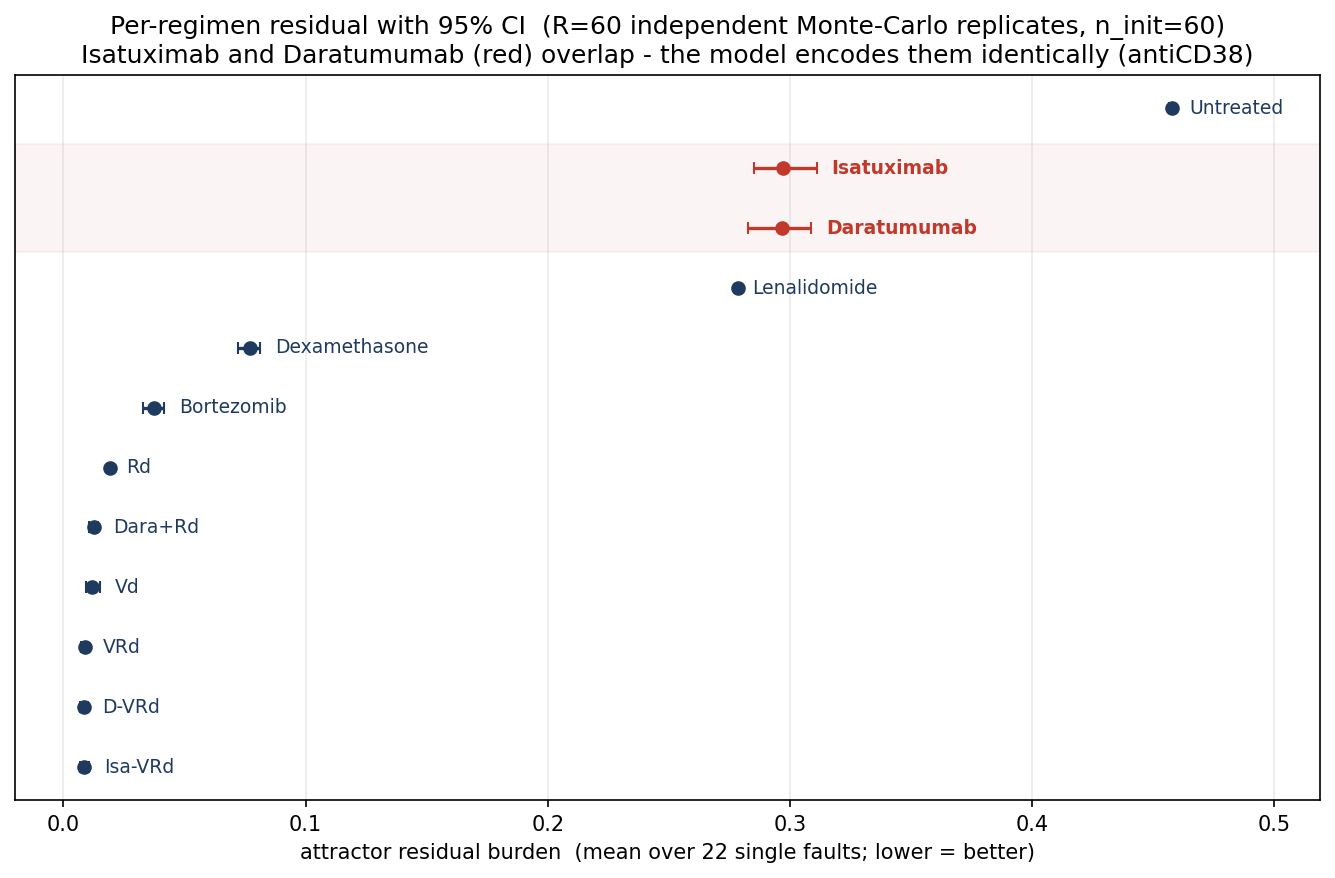
\includegraphics[width=\linewidth]{MM_attractor_ci.png}
\caption{Per-regimen residual with $95\%$ CIs over independent Monte-Carlo
replicates. Isatuximab and Daratumumab (red) overlap.}
\label{fig:ci}
\end{figure}

\subsection{Sensitivity and robustness}\label{sec:res-sens}
\textbf{Update scheme.} Because synchronous updating can create spurious cycles,
we re-ran every condition under random-asynchronous updating from matched initial
states. The absorbing death state satisfies $\text{step}(s)=s$, so it is a fixed
point under any order and cannot be a synchronous artifact; empirically $95\%$ of
synchronous attractors are already fixed points (the rest $2$-cycles), and all
$338$ sampled fixed points---including every death state---are asynchronous fixed
points. The two schemes agree on survive/die for $96\%$ of conditions, keep the
residual essentially unchanged for co-surviving cells ($r=0.97$), preserve
apoptotic reachability ($168/173$ death-dominant conditions), and---most
importantly---preserve the regimen ranking (Spearman $\rho=1.00$ on residual,
$0.99$ on apoptotic propensity; $\rho\ge0.97$ across seeds). The only shift is a
modest drop in anti-CD38 \emph{monotherapy} death propensity ($0.49\!\to\!0.38$),
which does not change the ranking.

\textbf{Rule and structure.} Perturbing the model one choice at a time---removing
each restored feedback edge (MYC$\to$IRF4, IRF4$\to$MYC, IRF4$\to$MCL1) or the
apoptosis latch, and flipping OR$\leftrightarrow$AND at each fused node---leaves
the ranking robust (median Spearman $\rho=0.96$ over $16$ perturbations;
$\rho\ge0.94$ for every feedback-edge removal). Its only real sensitivity is to
the death-decision operators (pro-apoptotic union $\rho\approx0.81$, BH3 guard
$\rho\approx0.73$), as expected for a survival readout. The same perturbations localize the two multistabilities (Sec.~\ref{sec:res-attr}).

\textbf{Readout.} Dropping any one of the eight outputs, or squaring the load,
leaves the ranking essentially unchanged (Spearman $\rho\ge0.97$; best regimen
preserved); it is most sensitive to hard binarization at $0.5$ ($\rho\approx0.82$),
which collapses the near-tied top regimens, so the continuous score is what
resolves among them. With the stable Monte-Carlo intervals of Fig.~\ref{fig:ci},
these checks show the ordering is a property of the network logic, not of the
update scheme, the rules, or the readout.

\subsection{Baselines and null models}\label{sec:res-baseline}
Two controls test whether the ranking is a property of the network logic rather
than of regimen size. A drug-count baseline (rank by number of agents) correlates
with the model ($\rho=0.86$ against mean residual) but has \emph{no} within-stratum
resolution: among the four single agents the model spans $0.036$--$0.278$
($7.7\times$) while the baseline calls them equal, and the best three-drug regimen
ties the best four-drug one. A randomized-rule null ($N{=}200$; identical topology
and drug-action points, Boolean operators and input signs shuffled) does
\emph{not} reproduce this---$\rho(\text{null},-\text{count})=0.05$ (only $0.5\%$ of
nulls reach the model's $0.86$), and only $8.5\%$ reproduce all three clinical
facts the model gets right (bortezomib the best single agent, bortezomib $<$
dexamethasone, VRd on top). The drug-count correlation is therefore a
\emph{consequence} of the logic, not a confound.

\subsection{Literature concordance}\label{sec:res-novel}
Because the model is not fit to outcomes, we can ask whether its predictions
independently agree with the literature (Table~\ref{tab:concordance}). Of eight
tests spanning regimen ranking (A1--A3) and fault-level vulnerability (C1--C4),
six are concordant and two (A1, B1) are affected by the intrinsic scope rather
than concordant: the VRd backbone tops the ranking, bortezomib outranks dexamethasone, lenalidomide is weak alone but strong
in combination, and the hardest genotypes---STAT3, MCL1/1q21 gain, BCL-2-high,
TP53 loss, RAS---are those flagged clinically as high-risk. The two scope-affected entries share one cause. For A1 the model
scores D-VRd \emph{equal} to VRd because anti-CD38 is subsumed in any Btz/Dex
backbone (Sec.~\ref{sec:res-ci}), whereas PERSEUS reports D-VRd improves PFS; for
B1 it ranks anti-CD38 the \emph{weakest} single agent, whereas daratumumab
monotherapy is clinically active. Both follow from omitting immune effectors
(ADCC/ADCP/CDC)---a consistent scope check that localizes anti-CD38's benefit to
the excluded compartment. This is a consistency
check, not patient-data validation; a genotype-matched test
(Sec.~\ref{sec:val}) remains future work.

\begin{table}[t]
\centering
\scriptsize
\caption{Literature concordance (C $=$ concordant, S $=$ intrinsic-scope limit).}
\label{tab:concordance}
\setlength{\tabcolsep}{3pt}
\begin{tabular}{@{}p{0.04\linewidth} >{\raggedright\arraybackslash}p{0.45\linewidth} >{\raggedright\arraybackslash}p{0.35\linewidth} c@{}}
\toprule
 & Model prediction & Evidence & \\
\midrule
A1 & VRd $=$ anti-CD38+VRd (subsumed) & D-VRd improves PFS~\cite{perseus,castor,pollux} & S \\
A2 & bortezomib $>$ dexamethasone & APEX trial~\cite{apex} & C \\
A3 & lenalidomide weak alone, strong in combination & clinical use in Rd/VRd~\cite{perseus,relapse} & C \\
B1 & anti-CD38 weakest single agent & daratumumab ORR $\sim$31\%~\cite{gen501,sirius} & S \\
C1 & STAT3-driven disease hardest & STAT3 survival signaling~\cite{stat3,shaffer} & C \\
C2 & MCL1-high (1q21) harder & 1q21 gain poor prognosis~\cite{imwghr} & C \\
C3 & BCL-xL/BCL-2-high raises survival & venetoclax in t(11;14)~\cite{venetoclax} & C \\
C4 & TP53 loss and RAS high-risk & del(17p), RAS~\cite{imwghr} & C \\
\bottomrule
\end{tabular}
\end{table}

\subsection{Enabled analysis: automatic test-pattern generation}\label{sec:res-atpg}
The FSM/HDL view treats combination discovery as test generation: a combination
is a test pattern, and a fault is \emph{detected} when the pattern drives the
absorbing APOP state from every sampled initial condition. Because the effective
drug space is small (four agents, $16$ patterns), exhaustive ATPG is complete
rather than heuristic. Of the $22$ faults, $21$ are detectable and one---%
constitutive STAT3---is \emph{undetectable} (no pattern exceeds apoptotic
propensity $0.56$), because STAT3 sustains BCL-xL while blunting the BIM arm, so
neither the NOXA (bortezomib) nor BIM (dexamethasone) route lifts the guard; this
independently recovers the STAT3 vulnerability of Table~\ref{tab:concordance}
(C1). Each detectable fault is killed by a single agent, but no single agent
covers all (bortezomib $19/22$, dexamethasone $16/22$); their union
bortezomib$+$dexamethasone is the minimal pattern covering all $21$, as
NF-$\kappa$B/NOXA and BIM induction are complementary, while anti-CD38 and
lenalidomide are not required for intrinsic coverage. Coverage and depth are
distinct axes: ATPG asks \emph{coverage} (can a pattern drive every fault to death
above threshold) and answers bortezomib$+$dexamethasone, whereas the regimen
ranking asks \emph{depth} (how far residual burden is suppressed), where that same
pair ranks last among the tabled regimens (Table~\ref{tab:rank}). The two do not
conflict---a two-drug pattern can detect every fault yet leave more residual
signaling than VRd---and this is why clinical practice, prioritizing depth of
response, uses the deeper three- and four-drug regimens rather than the minimal
covering pair. This model-internal proof of
concept---ignoring resistance evolution, subclones, pharmacokinetics, and the
immune axis---shows the framing turns combination search into a coverage problem;
with only $16$ patterns it demonstrates the framing rather than a computational
advantage.

%==============================================================================
\section{Discussion}\label{sec:disc}
Reading a mutation as a stuck-at fault, a drug as a fault-masking input, a
combination as a test pattern, and a cell fate as an attractor turns a Boolean MM
network into an object that equivalence checking, model checking, and ATPG act on
directly. The single-pass model is the combinational core; restoring the
IRF4--MYC loop and the absorbing latch makes it a sequential circuit whose
reachable states are cell fates, and exporting it as synthesizable Verilog makes
the analogy literal rather than rhetorical.

The dynamical extension is not cosmetic. Cell-fate multistability appears in
$24\%$ of conditions the acyclic single pass cannot represent, and the two models
disagree substantially (Fig.~\ref{fig:compare}). The perturbation analysis
(Sec.~\ref{sec:res-sens}) shows this is a genuine consequence of identified
elements---the IRF4--MYC loop generates the attractor multiplicity and the
BH3/latch logic the survive/die bistability---while the regimen ranking is
preserved under asynchronous update and single-rule and readout perturbations.
That the model, without being fit to any outcome, reproduces the VRd standard of
care and flags the clinically recognized high-risk genotypes
(Sec.~\ref{sec:res-novel}) is a further consistency check.

The value of the Verilog export should be stated carefully. At $22$ nodes,
exhaustive enumeration already suffices, so the export is not faster here; its
value is \emph{interface and scale}. Equivalence with the reference is verified,
and the same netlist can be handed unchanged to SAT- and model-checking-based
reachability~\cite{dubrova} and test-generation tools as networks grow beyond
enumeration. A quantitative comparison with time-frame-expanded Max-SAT
ATPG~\cite{linkhatri} on larger networks, and model-checking queries on the FSM
with off-the-shelf tools, are the next steps.

The model's boundaries are explicit and, in one case, diagnostic. It is
\emph{intrinsic}: it omits immune effector mechanisms (ADCC/ADCP/CDC), so it
underranks anti-CD38 monotherapy and treats isatuximab and daratumumab as one
input; the literature discordances (Sec.~\ref{sec:res-novel}) fall exactly where
the excluded biology dominates. It is single-clone, with microenvironmental
inputs at baseline, and Boolean and untimed, with no dose or pharmacokinetics.
Graded drug effects (multi-valued nodes), alternative latch formulations (e.g.,
requiring sustained pro-apoptotic input), most-permissive update semantics, and
non-uniform initial-state priors are open robustness questions beyond the
update-, rule-, and readout-level checks reported here. Above all, the regimen
rankings are \emph{in silico} mechanistic hypotheses: unlike prior work that
tested predictions in cell lines~\cite{vundavilli}, ours have not been evaluated
against patient, cell-line, or experimental response data, and the concordance of
Sec.~\ref{sec:res-novel} is a consistency check. Mapping genotypes to faults for
MM cell-line panels and genotype-matched patient cohorts (Sec.~\ref{sec:val}) is
the planned external validation.

%==============================================================================
\section{Conclusion}\label{sec:concl}
We recast a Boolean multiple-myeloma signaling network in the vocabulary of
digital-logic design---mutation as stuck-at fault, drug as input, combination as
test pattern, cell fate as attractor---and showed that the single-pass model is a
combinational circuit while restoring feedback and a clock yields a sequential
circuit / finite-state machine whose attractors expose a $24\%$ cell-fate
multistability the acyclic model cannot see. Monte-Carlo intervals quantify the
uncertainty and render the two anti-CD38 antibodies indistinguishable by
construction, and a synthesizable Verilog export, verified against the reference
over $20{,}000$ cases, opens the network to formal verification and ATPG. The
model reproduces the VRd standard of care and the recognized high-risk genotypes
without being fit to outcomes, and its regimen ranking is robust to update
scheme, individual rules, and readout; external validation against
genotype-matched patient response is the natural next step.

\section*{Reproducibility}
Code, the Verilog module and testbench, all figures, and the screening results
are available at \url{https://github.com/SangHoonChung/Mutations-as-Stuck-at-Faults}. A node-level model-provenance table,
the full attractor-residual heatmap, and the gate-level sequential-core schematic, the attractor state-transition
diagram, and the integrated pathway map are provided as online supplementary
material.



%==============================================================================
\begin{thebibliography}{9}
\bibitem{seer} National Cancer Institute, Surveillance, Epidemiology, and End
Results (SEER) Program. \emph{Cancer Stat Facts: Myeloma}.
\url{https://seer.cancer.gov/statfacts/html/mulmy.html} (accessed Oct.\ 2026).
\bibitem{acs} American Cancer Society. \emph{Key Statistics About Multiple
Myeloma}.
\url{https://www.cancer.org/cancer/types/multiple-myeloma/about/key-statistics.html} (accessed Oct.\ 2026).
\bibitem{globocan} F.~Bray et al. Global cancer statistics 2022: GLOBOCAN
estimates of incidence and mortality worldwide for 36 cancers in 185 countries.
\emph{CA Cancer J. Clin.}, 74(3):229--263, 2024.
\bibitem{relapse} S.~K.~Kumar et al. Multiple myeloma.
\emph{Nat. Rev. Dis. Primers}, 3:17046, 2017.
\bibitem{perseus} P.~Sonneveld et al. Daratumumab, Bortezomib, Lenalidomide,
and Dexamethasone for Multiple Myeloma (PERSEUS). \emph{N. Engl. J. Med.},
390:301--313, 2024.
\bibitem{cbm} A.~Grover et al. Computational modeling of protein networks
predicts treatment outcomes in multiple myeloma (MM). \emph{Blood},
130(Suppl.~1):592, 2017.   % ASH 2017 abstract -- CONFIRM first author
\bibitem{fumia} H.~F.~Fumi\`a and M.~L.~Martins. Boolean network model for
cancer pathways. \emph{PLoS ONE}, 8(7):e69008, 2013.
\bibitem{layek} R.~Layek, A.~Datta, M.~Bittner, and E.~R.~Dougherty. Cancer
therapy design based on pathway logic. \emph{Bioinformatics}, 27(4):548--555, 2011.
\bibitem{gsp} E.~R.~Dougherty and A.~Datta. Genomic signal processing: diagnosis
and therapy. \emph{IEEE Signal Process.\ Mag.}, 22(1):107--112, 2005.
\bibitem{linkhatri} P.-C.~K.~Lin and S.~P.~Khatri. Application of Max-SAT-based
ATPG to optimal cancer therapy design. \emph{BMC Genomics}, 13(Suppl.~6):S5, 2012.
\bibitem{vundavilli} H.~Vundavilli, A.~Datta, C.~Sima, J.~Hua, R.~Lopes, and
M.~Bittner. Targeting oncogenic mutations in colorectal cancer using
cryptotanshinone. \emph{PLoS ONE}, 16(2):e0247190, 2021.
\bibitem{stat3} R.~Catlett-Falcone et al. Constitutive activation of Stat3
signaling confers resistance to apoptosis in human U266 myeloma cells.
\emph{Immunity}, 10(1):105--115, 1999.
\bibitem{shaffer} A.~L.~Shaffer et al. IRF4 addiction in multiple myeloma.
\emph{Nature}, 454:226--231, 2008.
\bibitem{kronke} J.~Kr\"onke et al. Lenalidomide causes selective degradation
of IKZF1 and IKZF3 in multiple myeloma cells. \emph{Science},
343(6168):301--305, 2014.
\bibitem{kegg} M.~Kanehisa and S.~Goto. KEGG: Kyoto Encyclopedia of Genes and
Genomes. \emph{Nucleic Acids Res.}, 28(1):27--30, 2000.
\bibitem{kauffman} S.~A.~Kauffman. Metabolic stability and epigenesis in
randomly constructed genetic nets. \emph{J. Theor. Biol.}, 22(3):437--467, 1969.
\bibitem{thomas} R.~Thomas. On the relation between the logical structure of
systems and their ability to generate multiple steady states or sustained
oscillations. \emph{Springer Ser. Synergetics}, 1981.
\bibitem{pyboolnet} H.~Klarner, A.~Streck, and H.~Siebert. PyBoolNet: a Python
package for the generation, analysis and visualization of Boolean networks.
\emph{Bioinformatics}, 33(5):770--772, 2017.
\bibitem{ginsim} A.~Naldi et al. Logical modeling and analysis of cellular
regulatory networks with GINsim. \emph{Front. Physiol.}, 9:646, 2018.
\bibitem{maboss} G.~Stoll et al. MaBoSS 2.0: an environment for stochastic
Boolean modeling. \emph{Bioinformatics}, 33(14):2226--2228, 2017.
\bibitem{dubrova} E.~Dubrova and M.~Teslenko. A SAT-based algorithm for finding
attractors in synchronous Boolean networks. \emph{IEEE/ACM Trans. Comput. Biol.
Bioinform.}, 8(5):1393--1399, 2011.
\bibitem{testing} M.~L.~Bushnell and V.~D.~Agrawal. \emph{Essentials of
Electronic Testing for Digital, Memory and Mixed-Signal VLSI Circuits}.
Springer, 2000.
\bibitem{physiboss} G.~Letort et al. PhysiBoSS: a multiscale agent-based
modelling framework integrating physical dimension and cell signalling.
\emph{Bioinformatics}, 35(7):1188--1196, 2019.
\bibitem{cellnopt} C.~Terfve et al. CellNOptR: a flexible toolkit to train
protein signaling networks to data. \emph{BMC Syst. Biol.}, 6:133, 2012.
\bibitem{tait} S.~W.~G.~Tait and D.~R.~Green. Mitochondria and cell death:
outer membrane permeabilization and beyond. \emph{Nat. Rev. Mol. Cell Biol.},
11(9):621--632, 2010.
\bibitem{castor} A.~Palumbo, A.~Chanan-Khan, K.~Weisel, et al. Daratumumab,
bortezomib, and dexamethasone for multiple myeloma. \emph{N. Engl. J. Med.},
375(8):754--766, 2016.
\bibitem{pollux} M.~A.~Dimopoulos, A.~Oriol, H.~Nahi, et al. Daratumumab,
lenalidomide, and dexamethasone for multiple myeloma. \emph{N. Engl. J. Med.},
375(14):1319--1331, 2016.
\bibitem{apex} P.~G.~Richardson, P.~Sonneveld, M.~W.~Schuster, et al. Bortezomib
or high-dose dexamethasone for relapsed multiple myeloma. \emph{N. Engl. J.
Med.}, 352(24):2487--2498, 2005.
\bibitem{gen501} H.~M.~Lokhorst, T.~Plesner, J.~P.~Laubach, et al. Targeting CD38
with daratumumab monotherapy in multiple myeloma. \emph{N. Engl. J. Med.},
373(13):1207--1219, 2015.
\bibitem{sirius} S.~Lonial, B.~M.~Weiss, S.~Z.~Usmani, et al. Daratumumab
monotherapy in patients with treatment-refractory multiple myeloma (SIRIUS): an
open-label, randomised, phase 2 trial. \emph{Lancet}, 387(10027):1551--1560,
2016.
\bibitem{imwghr} P.~Sonneveld, H.~Avet-Loiseau, S.~Lonial, et al. Treatment of
multiple myeloma with high-risk cytogenetics: a consensus of the International
Myeloma Working Group. \emph{Blood}, 127(24):2955--2962, 2016.
\bibitem{venetoclax} S.~Kumar, J.~L.~Kaufman, C.~Gasparetto, et al. Efficacy of
venetoclax as targeted therapy for relapsed/refractory t(11;14) multiple
myeloma. \emph{Blood}, 130(22):2401--2409, 2017.

\end{thebibliography}

\end{document}
